% !TeX root = ../main.tex

\chapter{實際上排版玩看看}
\label{ch:start}

好了,現在正式來玩看看吧!本章主要是簡單的實例說明,先進入狀況再談其他。實際應用比高談闊論有用多了。

先來個「最高指導原則」:\textcolor{red}{\bfseries 學會控制空間,你就學會排版了}!剛學排版的朋友,往往會把所學到的東西去想法子佈滿你所有的空間(就是一個頁面),但實際上,你要調整的,其實是各個部份的空間配置,抽象一點說,也就是一整個頁面當中,沒有文字、圖表的部份才是排版真正的重點。你先聽聽就好,過一段時間的熟悉後,再來回頭思考這個「玩弄」空間的原則。:-)

由於本文有 HTML 版本,為了轉換上不造成失真,實例的部份,文稿上只寫程式碼,結果的部份都是編譯好的 PDF 格式檔案,置放於網站上,可線上閱覽或下載,簡單的例子則不另製作獨立的 PDF 檔,請參閱本文的 PDF 格式檔案內容。

\section{簡單的實例}

這裡就把前一章所談到的一些內容整理成一個文稿,先來試試看,這裡先使用 {\ttfamily report}\index{report@\texttt{report}} 類別文稿,因為 {\ttfamily article}\index{article@\texttt{article}} 類別文稿是沒有 {\ttfamily chapter} 的:

\begin{quote}
   \begin{verbatim}
% example1.tex
\documentclass{report}
\begin{document}
This is my first {\LaTeX} typesetting example.\\
This is my first \LaTeX{} typesetting example.\\
This is my first \LaTeX{} typesetting example.\\
I am Mr. Edward G.J. Lee, G.J. is a abbreviation of my name.\\
I am Mr.\ Edward G.J. Lee, G.J. is a abbreviation of my name.\\
Please see Appendix A. We will be there soon.\\
Please see Appendix A\null. We will be there soon.
\end{document}
\end{verbatim}
\end{quote}

使用編輯器編輯,然後存檔成 {\ttfamily exmaple1.tex},這樣就可以編譯了:

\begin{quote}
   \begin{verbatim}
latex example1.tex       => 產生 example1.dvi
dvips -Ppdf example1.dvi => 產生 example1.ps
ps2pdf example1.ps       => 產生 example1.pdf 或
dvipdfm[x] example1.dvi  => 由 example1.dvi 直接產生 example1.pdf 或
pdflatex example1.tex    => 由 example1.tex 直接產生 example1.pdf
\end{verbatim}
\end{quote}

編譯好的 PDF 檔可在此下載或閱覽:

\begin{quote}
   \url{http://edt1023.sayya.org/tex/latex123/example1.tex}  \\
   \url{http://edt1023.sayya.org/tex/latex123/example1.pdf}
\end{quote}

\subsection{關於換行}

每行最後加了個 \verb|\\|\index{\\@\verb=\\=},這表示強迫換行的意思,否則 \LaTeX{} 會依版面預設的寬度來換行,就不會是一個句子一行了,大家可以把這個 \verb|\\| 拿掉,再來編譯試看看結果,就會知道怎麼一回事了。也可以使用 \verb|\newline|\index{newline@\verb=\newline=} 這個指令,當然,我們都會聰明的選用較短的指令。而且 \verb|\\| 可以控制換行時的間隔,這在 \verb|\newline| 則不行。例如:

\begin{quote}
   \begin{verbatim}
Please see Appendix A. We will be there soon.\\[1cm]
Please see Appendix A\null. We will be there soon.
\end{verbatim}
\end{quote}

這樣的話,兩行之間的行距\index{行距}就是原來的行距再加上 {\ttfamily 1cm}。甚至,也可以是負數的參數,這樣行距就會變成原來的行距減去 {\ttfamily 1cm},當然,如果設過頭了的話,兩行可能會重疊在一起。既然,這裡使用的是方括號,表示這些參數是可以省略的。

另外,\verb|\linebreak[n]|\index{linebreak@\verb+\linebreak+} 也可以強迫換行\index{強迫換行},{\ttfamily n} 代表由 1--4 的建議值,數值愈大表示愈是強烈建議,不設定的話,就是換或不換兩種選擇,沒有中間地帶。和前面所說的不同處是,這種換行會把原來那一行句子的長度平均布滿版面上行寬的長度。例如:

\begin{quote}
   \begin{verbatim}
Please see Appendix A. We will be there soon.\linebreak
Please see Appendix A\null. We will be there soon.
\end{verbatim}
\end{quote}

排版後會表現成:

\begin{quote}
   Please see Appendix A. We will be there soon.\linebreak
   Please see Appendix A\null. We will be there soon.
\end{quote}

\subsection{關於縮排\index{縮排}}

第一行縮排了!這是因為我們完全沒有分章節,所以,\LaTeX{} 就把這些內容當做是引言的部份,依 \LaTeX{} 的安排,引言開頭是會縮排的。要解決這個問題,可有兩種方法:

\begin{enumerate}
   \item 在第一行之前加入 \verb|\noindent|\index{noindent@\verb+\noindent+} 來指示 \LaTeX{} 不要去縮排。但是這只作用在下指令的地方,其他該縮排的地方還是會縮排。
   \item 在 preamble 區加入 \verb|\parindent=0pt|\index{parindent@\verb+\parindent+},這表示讓全文的縮排為 {\ttfamily 0pt},當然,這就表示全文都不要縮排了。
\end{enumerate}

\section{加入章節標題\index{章節標題}}

在 \LaTeX{} 裡頭,要加入章節標題實在是太容易了,也不必去管字體的大小及置放的位置,盡管加上去就對了!\LaTeX{} 會替我們安排一切。我們這裡仍然以 {\ttfamily report} 類別來說明,因為 {\ttfamily article} 類別裡頭,沒有章,只能適用於較簡單的短文。

\begin{quote}
   \begin{verbatim}
% example2.tex
\documentclass{report}
\begin{document}
This is the first experience of \LaTeX.
\chapter{Aesop Fables}
\section{The Ant and the Dove}
An ant went to the bank of a river to quench its thirst, and
being carried away by the rush of the stream, was on the
point of drowning.
A Dove sitting on a tree overhanging the water plucked a
leaf and let it fall into the stream close to her. The Ant
climbed onto it and floated in safety to the bank.
\section{The Dog in the Manger}
A dog lay in a manger, and by his growling and snapping
prevented the oxen from eating the hay which had been
placed for them.
``What a selfish Dog!'' said one of them to his companions;
``he cannot eat the hay himself, and yet refuses to allow
those to eat who can.''
\chapter{The Eagle and the Arrow}
An eagle sat on a lofty rock, watching the movements of a
Hare whom he sought to make his prey.
An archer, who saw the Eagle from a place of concealment,
took an accurate aim and wounded him mortally.
\end{document}
\end{verbatim}
\end{quote}

編譯出來的結果:

\begin{quote}
   \url{http://edt1023.sayya.org/tex/latex123/example2.tex}\\
   \url{http://edt1023.sayya.org/tex/latex123/example2.pdf}
\end{quote}

請注意他什麼時候會縮排,什麼時候會換頁。{\ttfamily report} 類別,新的一章會換頁,如果想節省一點空間,可以換用 {\ttfamily article} 類別,\verb|\chapter{}| 改用 \verb|\section{}|,原來 \verb|\section{}| 就改用 \verb|\subsection{}|,這樣就不會換頁,內容就會連續下去了。大家可以試著把 {\ttfamily report} 改成 {\ttfamily article} 及 {\ttfamily book} 再重新編譯一次,試試看結果有何不同。

\section{加入 title page 資訊}
\label{sec:titlepage}\index{title page}

這是指內頁的第一頁,我也不知道這個中文專有名詞是什麼,在 \LaTeX{} 裡頭,我們就稱為 title page。在 \LaTeX{} 的標準格式裡,他包括了標題(title)、作者名字(author)、日期(date\index{date})及感謝詞(thanks\index{thanks})。要注意的是,在 {\ttfamily report/book} 類別,title page 是自成一單獨頁的,但在 {\ttfamily article} 類別裡,他是和本文連起來的。我們就以上面的伊索寓言的文章為例,要修改的地方是 preamble\index{preamble} 區及本文區的 \verb|\maketitle|\index{\verb=\maketitle=}:

\begin{quote}
   \begin{verbatim}
% example3.tex
\documentclass{report}
\title{Aesop Fables}
\author{Aesop\thanks{Thanks to the reader.}
      \and Nobody\thanks{Thanks to nobody.}}
\date{\today}
\begin{document}
\maketitle
This is the first experience of \LaTeX.
\chapter{Aesop Fables}
\section{The Ant and the Dove}
 ...
\end{verbatim}
\end{quote}

排版出來的結果如下:

\begin{quote}
   \url{http://edt1023.sayya.org/tex/latex123/example3.tex}\\
   \url{http://edt1023.sayya.org/tex/latex123/example3.pdf}
\end{quote}

我們可以發現,這一頁是不編頁碼的,從下一頁開始才是第一頁。作者可以有多個,使用 \verb|\and| 指令來連接。日期不一定要有,如果沒有 \verb|\date{\today}| 這個指令,那還是有日期,但只能固定在今天。如果內容過長,他會自動折行,但也可以手動加 \verb|\\| 來強迫換行,不管如何換行,整個句子是居中排列的。\verb|\maketitle| 是下在本文區的開頭,如果不下這個指令,那編譯時不會有什麼錯誤,只是就沒有 title page 了。

\section{加入目錄(Table of Contents)}
\label{sec;toc}

加入目錄(Table of Contents\index{Table of Contents})對 \LaTeX{} 而言,更是輕而易舉的事情,只要在本文開頭加個
\verb=\tableofcontents=\index{tableofcontents@\verb=\tableofcontents=}
指令就成了!依上面的例子,修改成:

\begin{quote}
   \begin{verbatim}
% example4.tex
\documentclass{report}
\title{Aesop Fables}
\author{Aesop\thanks{Thanks to the reader.}
      \and Nobody\thanks{Thanks to nobody}}
\date{\today}
\begin{document}
\maketitle
\tableofcontents
This is the first experience of \LaTeX.
\chapter{Aesop Fables}
\section{The Ant and the Dove}
 ...
\end{verbatim}
\end{quote}

排版出來的結果如下:

\begin{quote}
   \url{http://edt1023.sayya.org/tex/latex123/example4.tex}\\
   \url{http://edt1023.sayya.org/tex/latex123/example4.pdf}
\end{quote}

這裡千萬要注意的是,\verb|\tableofcontents| 要加在 \verb|\maketitle| 的後面,否則目錄會印在 title page 之前。而且要\textcolor{red}{\bf 編譯兩次}。第一次產生 {\ttfamily example4.toc},然後第二次編譯再跟據這個 {\ttfamily toc} 檔,真正編入目錄。

目錄是包括圖表目錄的(List of Figures, List of Tables),但我們目前還沒有談到圖表的排版,因此暫時略過,等談到時再來看要如何加入圖表目錄。

\section{加入摘要(abstract)}
\label{sec:abstract}\index{abstract}

這不一定會有,如果要加入的話,可使用 {\ttfamily abstract} 環境,在這個環境中的文章,左右會縮排。要注意的是,只有 {\ttfamily article/report} 類別才有 abstract,{\ttfamily book} 類別不能使用這個環境。

\begin{quote}
   \begin{verbatim}
% example5.tex
\documentclass{report}
\title{Aesop Fables}
\author{Aesop\thanks{Thanks to the reader.}
      \and Nobody\thanks{Thanks to nobody}}
\date{\today}
\begin{document}
\maketitle
\begin{abstract}
The tale, the Parable, and the Fable are all common and popular
modes of conveying instruction. Each is distinguished by its own
special characteristics.
\end{abstract}
\tableofcontents
\chapter{Aesop Fables}
\section{The Ant and the Dove}
 ...
\end{verbatim}
\end{quote}

排版出來的結果如下:

\begin{quote}
   \url{http://edt1023.sayya.org/tex/latex123/example5.tex}\\
   \url{http://edt1023.sayya.org/tex/latex123/example5.pdf}
\end{quote}

{\ttfamily report}\index{\texttt{report}} 類別的摘要自成一頁,不編頁碼,且不會編入目錄中,這和一般的論文格式可能會不一樣,使用時請注意。{\ttfamily artcile}\index{\texttt{artcile}} 的類別則仍然是和本文相連的,會出現在文章標題之後。

{\ttfamily abstract} 和 summary\index{summary} 在較正式的論文是有區分的,通常 abstract 在文前;summary 則在文後。但目前一般性的文章則沒有這樣區別,通通當成「摘要」。通常,摘要裡頭是不用註解、無交互參照也不使用公式圖表的。


\section{加入註解}
\label{sec:footnote}\index{註解}

在 \LaTeX{} 裡頭,註解可有兩種方式,一種是腳註(footnote)\index{footnote}\index{腳註},一種是邊註(marginal note)\index{marginal note}\index{邊註}。通常 \LaTeX{} 的腳註預設是由阿拉伯數字在編號,置於頁底部。在沒有部(part)的情形下,\texttt{report/book} 類別,編號每章會從頭起算,\texttt{article} 類別則會連續,而且,會使用 \texttt{footnotesize}\index{footnotesize@\texttt{footnotesize}} 的字體印出。邊註則不編號,字體是正常大小。

\subsection{腳註(Footnote)}

在所要加註的那個字後,使用 \verb|\footnote{}| 指令即可,解說的文字就寫入大括號之內,一般 \LaTeX{} 的指令在此都仍然有有作用,會印在此頁的底部,以小一點的字來印出,並加上編號。以下我們就試試看在 Dove 這個字來做腳註。請注意,Dove 這個字和 \verb|\footnote{}| 之間是沒有空白的。

\begin{quote}
   \begin{verbatim}
% example6.tex
\documentclass{report}
\title{Aesop Fables}
\author{Aesop\thanks{Thanks to the reader.}
      \and Nobody\thanks{Thanks to nobody}}
\date{\today}
\begin{document}
\maketitle
\tableofcontents
This is the first experience of \LaTeX.
\chapter{Aesop Fables}
\section{The Ant and the Dove}
An ant went to the bank of a river to quench its thirst, and
being carried away by the rush of the stream, was on the
point of drowning.
A Dove\footnote{Pigeon, an emblem of peace.}
sitting on a tree overhanging the water plucked a
leaf and let it fall into the stream close to her. The Ant
climbed onto it and floated in safety to the bank.
 ...
\end{verbatim}
\end{quote}

排版出來的結果如下:

\begin{quote}
   \url{http://edt1023.sayya.org/tex/latex123/example6.tex}\\
   \url{http://edt1023.sayya.org/tex/latex123/example6.pdf}
\end{quote}

\subsection{邊註(Marginal note)}

邊註只是把 \verb|\footnote{}| 換成 \verb|\marginpar{}|\index{marginpar@\verb=\marginpar=} 而已,內容仍然寫入大括號內。但和腳註不一樣的是,他沒有編號(因為就在旁邊,無此必要),他的字體也不會小一號,和內文的字體大小是一樣的,這在後面討論到字型的時候會談到如何改變字體的大小。

\begin{quote}
   \begin{verbatim}
% example7.tex
\documentclass{report}
\title{Aesop Fables}
\author{Aesop\thanks{Thanks to the reader.}
      \and Nobody\thanks{Thanks to nobody}}
\date{\today}
\begin{document}
\maketitle
\tableofcontents
This is the first experience of \LaTeX.
\chapter{Aesop Fables}
\section{The Ant and the Dove}
An ant went to the bank of a river to quench its thirst, and
being carried away by the rush of the stream, was on the
point of drowning.
A Dove\marginpar{Pigeon, an emblem of peace.}
sitting on a tree overhanging the water plucked a
leaf and let it fall into the stream close to her. The Ant
climbed onto it and floated in safety to the bank.
 ...
\end{verbatim}
\end{quote}

排版出來的結果如下:

\begin{quote}
   \url{http://edt1023.sayya.org/tex/latex123/example7.tex}\\
   \url{http://edt1023.sayya.org/tex/latex123/example7.pdf}
\end{quote}

\section{字型的相關調整}
\index{字型!相關調整}

\TeX/\LaTeX{} 的字型系統算是相當複雜的,這裡不多談其中原理,站在使用者的角度,我們只要知道怎麼使用就行了。在這裡,我們說字型(font)\index{font}\index{字型},指的是字型本身的一個總稱,或稱為字體\index{字體},在字的形狀的時候,我們就稱為字形(font shape)\index{font shape}\index{字形}。

\LaTeX{} 使用的字型選字機制,以目前新版本的 \LaTeX{} 而言,是使用 1993 年發行的 NFSS(New Font Selection Scheme) 第二版為標準。當然,仍然是建立在 \TeX\ 字型機制的基礎上的,這已超出這篇文章的範圍。

\subsection{\LaTeX{} 對字型的屬性描述}
\label{subsec:font-attr}\index{字型!屬性描述}

在 \LaTeX{} 裡,對於字型的描述,使用了五種屬性來說明,這五種屬性,也是 \LaTeX{} 巨集中常要使用到的參數,甚至是錯誤訊息標示字型來源的時候,會把字型的這些屬性給顯示出來。

\begin{enumerate}
   \item 字型編碼(font encoding)\index{font encoding}\index{字型!字型編碼}\\
         這裡所謂的字型編碼,指的是各個個別的字在一個字型裡頭的排列順序及安排方式。原始的 \TeX\ 字型編碼我們就稱為 OT1(Old \TeX\ text encoding)\index{OT1},這是預設的,如果都不指定字型編碼,那所使用的就是 OT1 編碼。在目前新一代的字型編碼裡頭,字的安排方式及內容和 OT1 不一樣,例如
         T1\footnote{正式名稱是 Cork's \TeX\ extended text encoding 又稱為 Text Companion encoding。這裡的 T1 和 Type 1 字型規格\index{字型!字型規格}無關,他是字型編碼方式,他把字型裡頭有關一些重音符號字母單獨視為一個單獨的字,而非如 OT1 是由一般字母和重音符號組合而成。}\index{T1},這在往後提到改變字型編碼時會再談到,我們目前就不去調整字型編碼,使用預設的 OT1,其他的編碼這裡就不多談了。

   \item 字族(font family)\index{font family}\index{字族}\\
         指同一設計類型的字型集合的名稱,例如羅馬字族(roman)\index{roman}\index{羅馬字族}、打字機字族(typewriter)\index{typewriter}\index{打字機字族}等等,通常前面會冠上製作商或製作人的名稱,例如 Knuth\index{Knuth} 教授設計的,稱為 `Computer Modern Roman'\index{Computer Modern Roman},Adobe 公司製作的羅馬字族稱為 `Adobe Times'\index{Adobe Times}。我們預設使用的,當然就是 Knuth 教授所設計的 Computer Modern fonts。以下為一些例子:

         \begin{quote}
            \begin{tabular}{>{\ttfamily}ll}
               簡稱 & 代表意義                   \\
               \hline
               cmr  & Computer Modern Roman      \\
               cmss & Computer Modern Sans Serif \\
               cmtt & Computer Modern Typewriter
            \end{tabular}
         \end{quote}

   \item 字型系列(font series)\index{font series}\index{字型!字型系列}\\
         這是指字型的 weight(胖瘦)及 width(長扁)來區分的。例如粗、細字體,一般我們正常用的是 medium,粗體則是 bold。以下是一些例子:

         \begin{quote}
            \begin{tabular}{>{\ttfamily}ll}
               簡稱 & 代表意義      \\
               \hline
               m    & medium        \\
               b    & bold          \\
               bx   & Bold extended \\
               sb   & Semi-bold     \\
               c    & Condensed
            \end{tabular}
         \end{quote}

   \item 字形(font shape)\index{font shape}\index{字形}\\
         這個望文生義,就是字的形狀。例如意大利斜體(italic)\index{italic}\index{意大利斜體}、斜體(slant)\index{slant}\index{斜體}、small caps\index{small caps} 等等。以下是幾個例子:

         \begin{quote}
            \begin{tabular}{>{\ttfamily}ll}
               簡稱 & 代表意義                              \\
               \hline
               n    & 正常字(normal),指 upright 或 roman \\
               it   & Italic                                \\
               sl   & Slanted                               \\
               sc   & Small Caps                            \\
            \end{tabular}
         \end{quote}

   \item 字型大小(font size)\index{font size}\index{字型!字型大小}\\
         預設的字型大小是 10pt(10 point),十點字。不加單位的話,預設的就是 pt。請注意,非標準 \LaTeX{} 類別的預設字型大小可能會不一樣。
\end{enumerate}

我們對字型要調整改變的,就是這些字型屬性的設定值。\LaTeX{} 已設定好方便的指令給我們使用。

\subsection{調整字族、字型系列、字形的指令}
\label{subsec:font-command}

\linespread{1.0}
\small
\begin{tabular}[\textwidth]{lllll}
      & 字型                & 標準指令                & 宣告式指令(環境)      & 舊用法                  \\
   \hline
   字 & \textup{textup}     & \verb|\textup{textup}| & \verb|{\upshape textup}| &                         \\
   形 & \textit{italic}     & \verb|\textit{italic}| & \verb|{\itshape italic}| & \verb|{\it italic}| \\
      & \textsl{slant}      & \verb|\textsl{slant}| & \verb|{\slshape slant}| & \verb|{\sl slant}| \\
      & \textsc{small caps} & \verb|\textsc{small caps}| & \verb|{\slshape small caps}| & \verb|{\sc small caps}| \\
   \hline
   系 & \textmd{medium}     & \verb|\textmd{medium}| & \verb|{\mdseries medium}| &                         \\
   列 & \textbf{boldface}   & \verb|\textbf{boldface}| & \verb|{\bfseries boldface}| & \verb|{\bf boldface}| \\
   \hline
   字 & \textrm{roman}      & \verb|\textrm{roman}| & \verb|{\rmfamily roman}| & \verb|{\rm roman}| \\
   族 & \textsf{sans serif} & \verb|\textsf{sans serif}| & \verb|{\sffamily sans serif}| & \verb|{\sffamily sans serif}| \\
      & \texttt{typewriter} & \verb|\texttt{typewriter}| & \verb|{\ttfamilyfamily typewriter}| & \verb|{\ttfamily typewriter}| \\
\end{tabular}
\linespread{1.36}
\normalsize

先別嚇了一跳,這是有跡可循的。其中 upright, medium, roman 都是一樣的,這是一般的正常字,就不必麻煩去設定他了,除非是要在特定字型範圍裡頭,重新改變成正常字體。從前面所說的簡稱的字串,再和 text, family, series, shape 去配對來使用,這樣只要記得簡稱就行了,例如:italic 的就是 \verb|\textit{}|。不然也可以使用「偷吃步」的舊用法,其實這也不是什麼偷吃步,他是原始 Plain \TeX\index{Plain \TeX} 所定義的,在舊版的 \LaTeX{} 2.09 也相容他而沿用,並加以擴充。但如果使用舊用法,那有時組合式的表示時可能會無效,例如粗斜體這種粗體和斜體設定混合時,就無法產生粗斜體了,這時還是得乖乖使用正統標準 \LaTeX{} 的表示法。

要注意的是,大括號的位置,宣告式的指令,整個作用範圍是連指令一起包住的,他可以當成環境來使用,例如 \verb|\begin{itsahpe}|, \verb|\end{itshape}|,這樣在這個環境內的文字就通通會使用 italic 斜體,也可以不加參數使用,例如 \verb|\itshape|,這樣以下的文字通通會使用 italic 斜體,直至另一個改變字型的指令出現為止。標準指令的作用範圍則是當做指令的一個參數,這些參數是出現在指令後的大括號內的。現在就來實際編譯個例子試看看:

\begin{quote}
   \begin{verbatim}
% example8.tex
\documentclass{report}
\title{\bfseries Aesop Fables}
\author{Aesop\thanks{Thanks to the reader.}
      \and Nobody\thanks{Thanks to nobody}}
\date{\today}
\begin{document}
\maketitle
\tableofcontents
\chapter{Aesop Fables}
\section{The \textsl{Ant} and the \textsl{Dove}}
\itshape
An antwent to the bank of a river to quench its thirst, and
being carried away by the rush of the stream, was on the
point of drowning.
\upshape
A \textsl{Dove} sitting on a tree overhanging the water plucked a
leaf and let it fall into the stream close to her. The \textbf{\textsl{Ant}}
climbed onto it and floated in safety to the bank.
\section{The {\it Dog}\/ in the Manger}
A \textbf{\textit{dog}} lay in a manger, and by his growling and snapping
prevented the oxen from eating the hay which had been
placed for them.
``What a selfish Dog!'' said one of them to his companions;
``he cannot eat the hay himself, and yet refuses to allow
those to eat who can.''
\chapter{The \textsc{Eagle} and the Arrow}
An \textsc{eagle} sat on a lofty rock, watching the movements of a
Hare whom he sought to make his prey.
An archer, who saw the \textsc{Eagle} from a place of concealment,
took an accurate aim and wounded him mortally.
\end{document}
\end{verbatim}
\end{quote}

我們把 title page\index{title page} 的標題改成粗體(請注意,宣告式或舊用法,大括號是把指令和文字整個括住的),把 Dove 改成 slant 斜體,把 dog 改成 italic 粗斜體\footnote{請注意,這兩種斜體是不一樣的,slant 是一般正常的字,只是把他傾斜個角度而已,但 italic 則是另一種獨特的字型設計。},把 ant 改成 slant 粗斜體,把 eagle 改成 small caps。由於章節標題原本就會轉換成粗體,所以章節標題的部份,粗體就不必重複設了。

但這裡發現例子裡第二章標題中的 Eagle 並沒有改變字體,而且以 {\ttfamily latex} 編譯時會產生以下的錯誤(這些訊息也會在 {\ttfamily example8.log} 中找到):

\begin{quote}
   \begin{verbatim}
  ...
LaTeX Font Warning: Font shape `OT1/cmr/bx/sc' undefined
(Font)              using `OT1/cmr/bx/n' instead on input line 4.
  ...
LaTeX Font Warning: Some font shapes were not available, defaults substituted.
  ...
\end{verbatim}
\end{quote}

現在我們看到了前面所談的屬性簡稱,這在 \LaTeX{} 就會使用這種屬性來表示而發出訊息,這裡 \verb|OT1/cmr/bx/sc| 就表示了 OT1 編碼,Computer Modern Roman 字族,Bold extended 系列,而且是 small caps 形狀的字型,錯誤訊息顯示,他並沒有定義,因此,這個字型將會使用預設的字型來代替,這裡就是以 n 正常形狀的 bx 系列字型來替代。所以,字型指令並不是都可以隨意組合的,有些是根本就沒有這種字型,有些則是沒有用巨集去定義好,這樣 \LaTeX{} 就取不到字了,但別擔心,頂多就是使用預設的字型罷了!

另一個很奇怪的地方,就是第一章、第二節的標題,為什麼是 \verb|{\it Dog}\/ in the...}|?這個插入的 \verb|\/| 是什麼東西?這是 \TeX\ 系統調整斜體字(包括 iatlic 及 slanted)和正常字之間的空白的一個指令,稱為 italic correction\index{italic correction}。這樣,在斜體字和正常字之間的空白才會正常。那為什麼其他的斜體指令沒有加這個調整呢?這是因為 \LaTeX{} 巨集在設計時就有考慮到這個問題,所以 \verb|\textit{}| 這類標準指令都會自動調整 italic correction,不必由我們手動調整。

另外,章節標題本就會自動轉換成粗體,標題上的 dog 為什麼沒有變粗體?這在前面有提到過,這種舊用法有時是無法複合使用的,粗體又斜體的指令會用不上來。因此,建議盡量使用 \LaTeX{} 的第一種標準指令來改變字型。使用 \verb|{\it ...}| 或 \verb|{\itshape ...}|\footnote{宣告式指令可以複合使用,但仍然會需要手動做 italic correction。} 這種指令的話,就得時時注意 italic correction 的問題,也得注意是否可以複合使用指令的問題,所以,還是不要偷懶的好。:-)

後下是排版出來的結果:

\begin{quote}
   \url{http://edt1023.sayya.org/tex/latex123/example8.tex} \\
   \url{http://edt1023.sayya.org/tex/latex123/example8.pdf}
\end{quote}

\subsection{相對字型大小的調整}

接下來談最後一個字型大小屬性的調整,這在使用上比較單純,只要知道指令就可以馬上拿來使用。但是 \TeX{}/\LaTeX{} 系統中,談到字型,裡頭一堆地雷,例如前面談到正常的內文字型大小是 10pt,現在如果想製作海報,需要 64pt 的字的時候就會發現,設不出來了!正常 \LaTeX{} 的定義,字型的大小範圍是在 5--24.88pt 之間,超出這個範圍的字需要其他的 package 的幫忙。\footnote{這是 \LaTeX{} 本身巨集定義的問題,因為他主要是針對一般性文件及書籍,\TeX{} 本身的能力,可以讓字型放大到 2047pt。}

這裡我們先來看看內文 10pt 時各種字型大小指令、實際例子及其大小(這是相對大小,會隨內文預設字型大小而自動調整):\footnote{請注意,本文 pdf 格式內文使用 12pt 字型大小,列表及其中的例子,是由另外 10pt 預設字型大小所製作的 eps 圖檔引入,以免失真。}

\begin{quote}
   \centering
   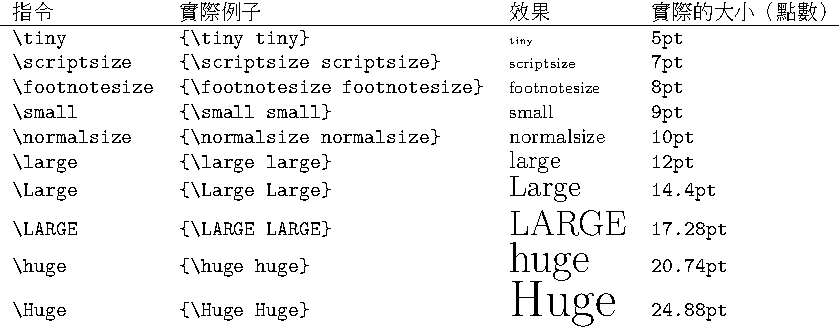
\includegraphics{fntsize}
\end{quote}

這些字型大小指令也可以當成環境來使用,例如:

\begin{quote}
   \begin{verbatim}
\begin{small}
  本文內容
\end{small}
\end{verbatim}
\end{quote}

這樣用也是可以的。

\subsection{絕對字型大小的調整}

通常字型的大小\index{字型!字型大小},使用上一節所說的相對字型大小來調整會比較方便,而且對於整個版面的配合也會比較恰當,例如行距也會跟著做適當的調整,如果自行用絕對字型大小的方法來調整字型大小的話,常常會造成行距不一致的情形,因此,如非必要,應盡量避免。

但有時候就是需要做這樣的調整,例如本文封面的字型大小,縱使是 \LaTeX{} 預設的最大字型也覺得稍小了點,這就要另外引入 package 調整了。

這裡我們使用 \textsf{type1cm}\index{type1cm@\textsf{type1cm}} package 來調整。當然,得使用 Type 1 字型,才可以達到無段放大、縮小的目的%
\footnote{\LaTeX{} 系統中的字型放大,在 10pt 以上,是以 1.2 的倍數為次方來放大的,因此,正文 10pt 的字型大小的話,不會有 13pt 這種大小的字型,\LaTeX{} 會選用最相近大小的字型來替代。}%
,而這個 package 也是配合 Type 1 字型使用的。個別放大的 pk 點陣字,這裡就不討論了,目前絕大部份的 Computer Modern 字型都已有 Type 1 的 free 版本,而且各個 \TeX\ distribution 都會附上,使用上會較方便。以下是 \textsf{type1cm} 的使用方法:

\begin{quote}
   \begin{verbatim}
  ...
\usepackage{type1cm}
  ...
\fontsize{字型大小}{行距大小}\seclectfont
  ...
\end{verbatim}
\end{quote}

還記得如何引用巨集套件\index{巨集套件}嗎?請參考第 \ref{ch:syntax} 章、第 \ref{sec:struct} 節,第 \ref{subsec:preamble} 小節的說明。

其中的「字型大小」就是所要指定的大小,通常以 pt 為單位,當然,要使用其他單位也是可以。「行距大小」也是要一併指定,不可省略。最後的 \verb|\seclectfont| 是讓他發生作用的意思,\LaTeX{} 有些關於字型的較低階指令,要下 \verb|\seclectfont| 後才會作用,\verb|\fontsize{}{}|\index{fontsize@\verb=\fontsize=} 正是其中之一。

\section{原文照列}

什麼是原文照列\index{原文照列}?一般 \LaTeX{} 遇到倒斜線\index{倒斜線}會認為是一個指令的開始,如果連整個指令都要印出的時候呢?這時就要用到原文照列的指令及環境了。

\subsection{原文照列指令}

如果只是一小段的文字要原文照列,那使用指令會比較方便,這個指令就是 \verb+\verb|文字內容|+\index{verb@\verb=\verb=},其中的 \verb+|+ 這個符號可以使用其他非字母的符號代替,只要前後相同就行了,例如:\verb|\verb+文字內容+| 這樣也是可以的。

\subsection{原文照列環境}

如果是一整段的內容要原文照列的話,使用環境會比較方便,那便是 {\ttfamily verbatim} 環境。不管是哪一種原文照列的情形,預設是使用打字機字族的字型來顯示的。底下是一個簡單的例子,說明原文照列指令及環境的使用:

% \begin{quote}
% \begin{Verbatim}[commandchars=+\[\]]

% \documentclass{article}
% \begin{document}
% The example of \verb|\verb{}| command and \texttt{verbatim} environment.
% \section{\textbackslash{}\texttt{verb} command}
% When you want to express you home directory, you can \verb|echo $HOME|
% varient to display your home directory in your sh script.
% \noindent
% \verb*|This is    4 space here.|
% \section{\texttt{verbatim} environment}
% Here is a sh script to determine if on GNU/Linux system.
% \begin{verbatim}
% #!/bin/sh
% Date=`date '+%y%m%d'`
% if [ `uname` = Linux ]
% then
%   Mail=/var/spool/mail/edt1023
%   Target=/mnt/hd
% else
%   Mail=/var/mail/edt1023
%   Target=/mnt/pub
% fi
% \end{verbatim}
% \end{document}
% \end{Verbatim}
% \end{quote}

這裡會發現一些奇怪現象,例如
\texttt{\textbackslash{}verb*}
那個星號是什麼意思呢?就是讓空白以 \verb*| | 的方式表示出來的意思,{\ttfamily verbatim} 環境也是可以這樣使用。例如 {\ttfamily example9} 中的:

\begin{quote}
   \begin{verbatim}
\verb*|This is    4 space here.|
\end{verbatim}
\end{quote}

也可以寫成:

% \begin{quote}
% \begin{Verbatim}[commandchars=+\[\]]
% \begin{verbatim*}
% This is    4 space here.
% \end{verbatim*}
% \end{Verbatim}
% \end{quote}

差別在於,環境的上下行會多空出個空白行出來。

另外,標題為什麼不使用 \verb+\verb|\verb|+ 就好了呢?原因是原文照列的指令和環境都不能當做其他指令的參數,標題本身就是一個指令,所以 \verb+\verb+ 不能在裡頭。

使用 \verb|\textbackslash|\index{textbackslash@\verb=\textbackslash=} 這麼長的敘述,而不用 \verb|$\backslash$| 這個簡單的方式,原因是這個文稿有使用 \LaTeX{}2{\ttfamily HTML} 來轉成 HTML 格式,使用 \LaTeX{} 的替代表示法會轉成一般的符號,但使用後者的方式則會轉成圖檔,所以這裡就使用 \LaTeX{} 的替代表示法了。

底下是排版出來的結果:

\begin{quote}
   \url{http://edt1023.sayya.org/tex/latex123/example9.tex} \\
   \url{http://edt1023.sayya.org/tex/latex123/example9.pdf}
\end{quote}

\section{加入中文}

這裡只說明如何使用 \textsf{CJK}\index{CJK@\textsf{CJK}} package 的情形,原因是一般 \TeX{} distribution 會附上(有些發行套件並沒有附上,這時只好自行安裝了)。\textsf{CJK} package 是把中文的部份包在一個環境裡頭,在這個環境內就可以使用中文,離開這個環境就又回復到原本的英文環境,底下由例子來說明。

\begin{quote}
   \begin{verbatim}
\documentclass{article}
\usepackage{CJK}  % 使用 CJK 巨集套件
\begin{document}
% 進入 CJK 環境,並使用 Big-5 碼及 hwmm 這個字型
\begin{CJK}{Bg5}{hwmm}
\section{CJK 巨集套件}
這是一個測試,關於 CJK package 的測試。
\section{桃花源記節錄}
初狹,纔通人;復行數十步,豁然開朗。土地平曠,屋舍儼然。有良田、美池、%
桑、竹之屬,阡陌交通,雞犬相聞。其中往來種作,男女衣著,悉如外人;黃髮、%
垂髫, 並怡然自樂。見漁人,乃大驚,問所從來;具答之,便要還家,設酒、殺雞、%
作食。村中聞有此人,咸來問訊。自云:「先世避秦時亂,率妻子邑人來此絕境,%
不復出焉;遂與外人閒隔。」問今是何世;乃不知有漢,無論魏、晉。此人一一%
為具言所聞,皆歎惋。餘人各復延至其家,皆出酒食。停數日,辭去。此中人語%
云:「不足為外人道也。」
\end{CJK}
\end{document}
\end{verbatim}
\end{quote}

就這麼簡單。只是編譯要改由 {\ttfamily bg5latex}\index{bg5latex@\texttt{bg5latex}} 而不是原來的 {\ttfamily latex} 指令,這是為了避開我們 Big-5 碼的一些特殊碼的關係,還記得為何每行最後要加個百分號 \verb|%|\index{%@\verb=%=} 嗎?這樣才不會插入英文的字間空白。編譯好的例子如下:

\begin{quote}
   \url{http://edt1023.sayya.org/tex/latex123/example10.tex} \\
   \url{http://edt1023.sayya.org/tex/latex123/example10.pdf}
\end{quote}

詳細的 \textsf{CJK} package 的使用中文說明,請參考 \textsf{CJK} package 所附的文件及〈我的 CJK〉一文:

\begin{quote}
   \url{http://edt1023.sayya.org/tex/mycjk/mycjk.html} \\
   \url{http://edt1023.sayya.org/tex/mycjk/mycjk.pdf}
\end{quote}